\documentclass{article}
\usepackage{graphicx}
\usepackage[top=1in, bottom=1in, left=1in, right=1in]{geometry}

\begin{document}

\title{Text Technologies for Data Science: Assessment 2}
\author{s1107496}

\maketitle

\section{Introduction}
This report describes the implementation of two information retrieval algorithms, brute.py and index.py, as well as refinements to the latter as implemented in best.py.

\section{brute.py and index.py}
\subsection{brute.py}
In brute.py, each news story was first transformed to lowercase and tokenized on whitespace, following which the tf-idf weighted cosine denominator component for the story was computed. Then, for every prior story, the tf-idf weighted cosine was calculated, drawing from both a pre-computed dictionary of token idf scores and a list-based cache of tokenized story/tf-idf weighted cosine denominator component tuples. In this way, only the query-document-unique numerator of the tf-idf weighted cosine formula needed to be calculated (for all tokens in both the query and document).  If the score of the best matching document exceeded the given threshold, the result was written to a file and immediately flushed. Finally, the token/denominator tuple for the latest news story was added to the aforementioned cache.
\subsection{index.py}
index.py improved upon brute.py by implementing a term-at-a-time indexing. The index was represented as a dictionary with tokens as keys and lists of story number/token count tuples as values. As in brute.py, tf-idf weighted cosine denominators were also cached for each story. When calculating tf-idf weighted cosine, partial story scores were stored in a dictionary. For 10,000 stories, index.py ran roughly 3.5 times faster than brute.py.

\section{best.py}
best.py included a number of refinements over index.py, as listed below. For 10,000 stories, best.py ran 17.7 times faster than index.py (62.8 times faster than brute.py). As measured against the provided pairs.ref, best.py had an accuracy of 91.13\%.
\subsection{Stop word removal}
After initial tokenization, all tokens from the English-language stop word list provided by \texttt{nltk} were removed. Additionally, domain-specific stop words (where idf < 3.38211) were removed. This increased speed by 10.34 times (measured on 10,000 stories), while lowering accuracy by 8.87\%. An additional speed improvement of 9.5\% could have been made at the expense of a further 0.78\% loss of accuracy, but this was deemed too likely to result in overfitting stop words to the given data.
\subsection{Identical story checking}
A large number of ...
\subsection{Pre-calculation of token idf}
(counter idf)
\subsection{Python-specific improvements}
In both documents and queries, to capture meaningful pairings of words, bigrams from the stop-word-sanitized token list were themselves added to the token list. This improved average precision by 0.0033, and was found to be more effective than trigrams or both bigrams and trigrams.

\section{Comparison of algorithm running times}
%\begin{figure}[ht!]
%\centering
%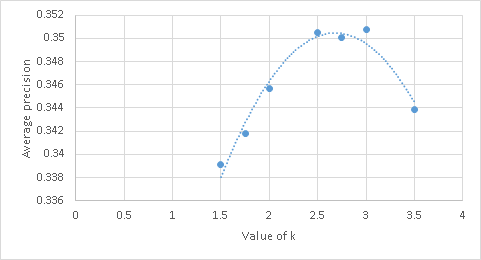
\includegraphics[width=90mm]{k_graph2.png}
%\end{figure}


\end{document}